\chapter{Problèmes rencontrés et limites}

\section{Les vidéos à annoter}

\subsection{Le live}

Nous avons testé notre programme seulement sur des vidéos en
replay, nous ne savons pas comment réagi le problème à un flux
vidéo en direct.
\bigskip

Nous savons en revanche que l'outil de base de visionnage fourni
par le client \textit{basic\_monitoring} fonctionne en live. Nous
pensons que notre programme peut fonctionner en live sans
problème mais peut-être avec du délai dans les annotations
(surtout si l'utilisateur veut annoter plusieurs vidéos en même
temps et ajouter la transparence).
\bigskip

\subsection{Taille des vidéos}

Une limite imposée par le code du client est la taille des
vidéos. Elles doivent impérativement être en format 640*480. 

Il est possible de lire des vidéos en dehors de ce format si on
désactive l'affichage des lignes du terrain, mais dans ce cas les
annotations affichées seront inexactes.
\bigskip

Comme nous pouvons le voir dans les deux images ci-dessous
(Figure~\ref{fig:sizevideo}), le décalage est nettement visible
pour la vidéo b, trop large par rapport au format demandé. La
position du robot 4 et sa target sont décalés par rapport au
robot et aux lignes du terrain

\begin{figure}[H]
    \centering
    \subfloat[640 x 480 vidéo]{
        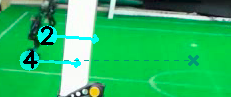
\includegraphics[scale = 0.7]{images/sizecorrect.png}
    }
     \qquad
    \subfloat [720 x 480 vidéo]{
        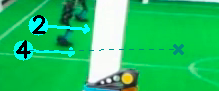
\includegraphics[scale = 0.7]{images/sizewrong.png}
    }
    \caption{Différence d'annotation en fonction de la taille de
    la vidéo}
    \label{fig:sizevideo}
\end{figure}

\subsection{Format des vidéos}

Nous avons pu tester différents formats de vidéo (avi, mov, mp4).
Ils sont tous les trois acceptés par OpenCV. Nous avons observé
des différences de performances suivant le format, nous avons
donc effectué des tests.

\bigskip

Le test est expliqué en partie~\ref{testperf},
page~\pageref{testperf}). 
\bigskip

Ces tests confirment bien une différence de performance des
codecs.
Si la charge de traitement est importante, nous conseillons donc
d'utiliser le format avi comme proposé dans les dossiers de vidéo
du drive.
\bigskip

Enfin, nous ne prenons pas en charge les vidéos dynamiques, elles
ne seront pas annotées. Pour la vidéo dynamique, la condition
\textbf{isFullySpecified()} n'est pas remplie. La vidéo étant en
perpétuel mouvement, nous ne pouvons pas (dans l'état actuel du
programme) recalculer d'équation de plan.
\bigskip

Pour les vidéo grand angle (par exemple ptgrey.avi dans les
vidéos du 20/02/2019 et du 21/03/2019) des annotations parfois
inextactes (voir Figure~\ref{fig:field},
page~\pageref{fig:field}).

\section{La transparence}
Nous souhaitions utiliser des annotations plus ou moins
transparentes (principalement pour la trace mais également pour
d'autres). 
\bigskip

Malheureusement, les fonctions de dessin d'OpenCV ne gèrent pas
la transparence. OpenCV gère bien les images avec transparence,
les fonctions de dessin acceptent des couleurs avec transparence,
mais lors du dessin, elles ignorent cette valeur, ne considèrent
que les canaux R,G,B et dessinent donc en opacité maximale.
\bigskip

La solution trouvée (qui semble être la seule proposée par
OpenCV) est le blend d'images entre elles (voir
\ref{transparence}).



\section{Le slider}

Pour implémenter un slider qui permette de choisir un moment dans
la vidéo, il est nécessaire de connaître certaines
caractéristiques de celle-ci : Soit le nombre total d'images et
le nombre d'images par seconde, soit la durée totale de la vidéo
et le nombre d'images par seconde. 
\bigskip

Dans un premier temps nous avons voulu utiliser le nombre total
d'images, mais le framerate des vidéos encodées par les clients
(30fps dans la plupart des cas) n'est pas constant, avec parfois
moins de 30 images sur une seconde. Dans ce cas, certaines images
sont dupliquées dans le fichier vidéo pour maintenir la
fréquence. 
\bigskip 

Mais ces images "doublons" ne sont pas comptabilisées dans le
nombre total d'image. On ne pouvait donc pas précisément définir
la durée de la vidéo.

La conséquence était un slider qui finissait sa course alors
qu'il restait une portion non négligeable de la vidéo à lire
(jusqu'a 50\% dans nos vidéos de test).
\bigskip

Le nombre d'images dupliquées dépend de la vidéo, et est dû
(pensons-nous) à un manque de puissance au niveau de l'ordinateur
l'ayant encodé lors de la capture. 

C'est pourquoi notre slider a donc été implémenté grâce aux
time\_stamp des images.

\section{La trace}

Il a été très difficile de stocker les anciennes positions de
manière optimisée.

Nous avons au début créé une queue. Pour afficher la trace on
affichait la première position puis on l'insérait à la fin
jusqu'à avoir parcouru toutes les positions et revenir à la
position initiale. 
\bigskip

Cette méthode n'était plus adaptée une fois le slider implémenté.
En effet, la queue ne permettait pas du tout le retour en
arrière. Si l'utilisateur effectuait un retour en arrière, il
était impossible d'afficher correctement la trace et il fallait
recommencer son affichage à partir de la position actuelle. 
\bigskip

Nous avons donc implémenté une map où l'on stocke les positions
en fonction de leur \textit{time\_stamp}. Cette méthode a
fonctionne parfaitement avec le slider. 

Lorsque nous parcourons la vidéo, nous stockons la position dans
la map et nous affichons toutes les positions dont le
\textit{time\_stamp} est compris entre le temps actuel et le
nombre de seconde précédent en fonction du nombre de
\textit{delay\_old\_pos} choisi par l'utilisateur.
\bigskip

Nous ne supprimons donc jamais les anciennes positions des robots
afin d'avoir un affichage optimisé dans l'interface. Mais cette
mémoire importante n'affecte pas à priori les performances, pour
les vidéos sur lesquelles nous l'avons testé.

